\documentclass[border=4pt]{standalone}

\usepackage{amsmath}
\usepackage{tikz}
\usepackage{mathdots}
\usepackage{yhmath}
\usepackage{cancel}
\usepackage{color}
\usepackage{siunitx}
\usepackage{array}
\usepackage{multirow}
\usepackage{amssymb}
\usepackage{gensymb}
\usepackage{tabularx}
\usepackage{booktabs}
\usetikzlibrary{fadings}
\usetikzlibrary{patterns}


\begin{document}
 

\tikzset{every picture/.style={line width=0.75pt}} %set default line width to 0.75pt        

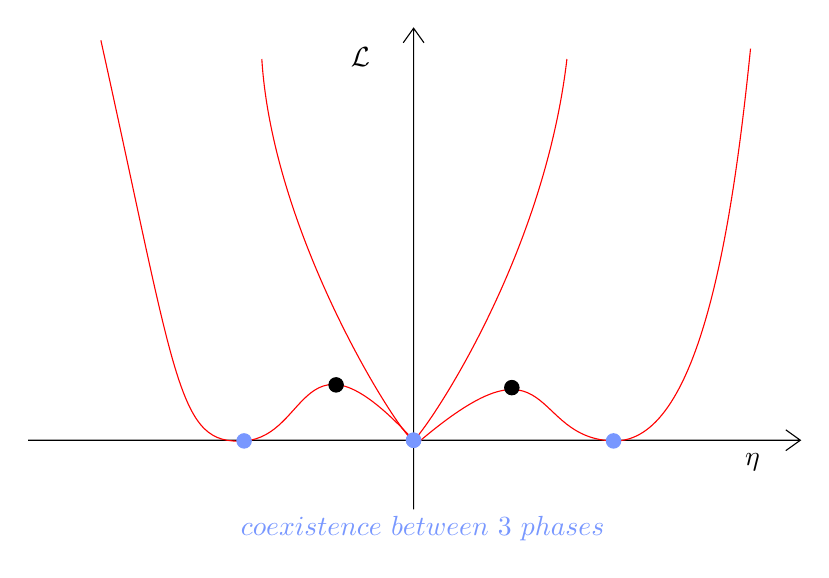
\begin{tikzpicture}[x=0.75pt,y=0.75pt,yscale=-1,xscale=1]
%uncomment if require: \path (0,300); %set diagram left start at 0, and has height of 300

%Shape: Axis 2D [id:dp867200198649551] 
\draw  (103,222.67) -- (475,222.67)(288.67,24.17) -- (288.67,256) (468,217.67) -- (475,222.67) -- (468,227.67) (283.67,31.17) -- (288.67,24.17) -- (293.67,31.17)  ;
%Curve Lines [id:da21533859561424595] 
\draw [color={rgb, 255:red, 255; green, 0; blue, 0 }  ,draw opacity=1 ]   (138,30) .. controls (175,197) and (175,225) .. (207,223) .. controls (239,221) and (234,163) .. (288.67,222.67) ;


%Shape: Circle [id:dp30843710460142804] 
\draw  [fill={rgb, 255:red, 0; green, 0; blue, 0 }  ,fill opacity=1 ] (247.88,196) .. controls (247.88,194.09) and (249.42,192.54) .. (251.33,192.54) .. controls (253.24,192.54) and (254.79,194.09) .. (254.79,196) .. controls (254.79,197.91) and (253.24,199.46) .. (251.33,199.46) .. controls (249.42,199.46) and (247.88,197.91) .. (247.88,196) -- cycle ;
%Curve Lines [id:da9720185755988506] 
\draw [color={rgb, 255:red, 255; green, 0; blue, 0 }  ,draw opacity=1 ]   (292.12,222.67) .. controls (357,168) and (344,222) .. (385,223) .. controls (426,224) and (442,123) .. (451,34) ;


%Shape: Circle [id:dp46719671724679235] 
\draw  [color={rgb, 255:red, 120; green, 151; blue, 255 }  ,draw opacity=1 ][fill={rgb, 255:red, 120; green, 151; blue, 255 }  ,fill opacity=1 ] (285.21,222.67) .. controls (285.21,220.76) and (286.76,219.21) .. (288.67,219.21) .. controls (290.58,219.21) and (292.12,220.76) .. (292.12,222.67) .. controls (292.12,224.58) and (290.58,226.13) .. (288.67,226.13) .. controls (286.76,226.13) and (285.21,224.58) .. (285.21,222.67) -- cycle ;
%Shape: Circle [id:dp8567054706937798] 
\draw  [color={rgb, 255:red, 120; green, 151; blue, 255 }  ,draw opacity=1 ][fill={rgb, 255:red, 120; green, 151; blue, 255 }  ,fill opacity=1 ] (203.54,223) .. controls (203.54,221.09) and (205.09,219.54) .. (207,219.54) .. controls (208.91,219.54) and (210.46,221.09) .. (210.46,223) .. controls (210.46,224.91) and (208.91,226.46) .. (207,226.46) .. controls (205.09,226.46) and (203.54,224.91) .. (203.54,223) -- cycle ;
%Shape: Circle [id:dp5965136232703812] 
\draw  [color={rgb, 255:red, 120; green, 151; blue, 255 }  ,draw opacity=1 ][fill={rgb, 255:red, 120; green, 151; blue, 255 }  ,fill opacity=1 ] (381.54,223) .. controls (381.54,221.09) and (383.09,219.54) .. (385,219.54) .. controls (386.91,219.54) and (388.46,221.09) .. (388.46,223) .. controls (388.46,224.91) and (386.91,226.46) .. (385,226.46) .. controls (383.09,226.46) and (381.54,224.91) .. (381.54,223) -- cycle ;
%Shape: Circle [id:dp17263285116353666] 
\draw  [fill={rgb, 255:red, 0; green, 0; blue, 0 }  ,fill opacity=1 ] (332.54,197.33) .. controls (332.54,195.42) and (334.09,193.88) .. (336,193.88) .. controls (337.91,193.88) and (339.46,195.42) .. (339.46,197.33) .. controls (339.46,199.24) and (337.91,200.79) .. (336,200.79) .. controls (334.09,200.79) and (332.54,199.24) .. (332.54,197.33) -- cycle ;
%Curve Lines [id:da9726920598487578] 
\draw [color={rgb, 255:red, 255; green, 0; blue, 0 }  ,draw opacity=1 ]   (215.54,39) .. controls (221,127) and (285,224.33) .. (288.67,222.67) .. controls (292.33,221) and (351,138) .. (362.54,39) ;


%Shape: Circle [id:dp3329242003091928] 
\draw  [color={rgb, 255:red, 120; green, 151; blue, 255 }  ,draw opacity=1 ][fill={rgb, 255:red, 120; green, 151; blue, 255 }  ,fill opacity=1 ] (285.21,222.67) .. controls (285.21,220.76) and (286.76,219.21) .. (288.67,219.21) .. controls (290.58,219.21) and (292.12,220.76) .. (292.12,222.67) .. controls (292.12,224.58) and (290.58,226.13) .. (288.67,226.13) .. controls (286.76,226.13) and (285.21,224.58) .. (285.21,222.67) -- cycle ;

% Text Node
\draw (263,38.17) node    {$\mathcal{L}$};
% Text Node
\draw (452,233.17) node    {$\eta $};
% Text Node
\draw (293,265) node  [color={rgb, 255:red, 120; green, 151; blue, 255 }  ,opacity=1 ]  {$coexistence\ between\ 3\ phases$};


\end{tikzpicture}


\end{document}
